\documentclass[final]{beamer}
\usepackage[T1]{fontenc}
\usepackage[utf8]{inputenc}
\usepackage[ngerman]{babel}
\usepackage{amsmath}
\usepackage{amsfonts}
\usepackage{amssymb}
\usepackage{graphicx}
\usepackage{color}
\usepackage{listings}


\setbeamercovered{transparent}

\setbeamertemplate{footline}{
	\setbeamercolor{section in head/foot}{fg=gray!20!white,bg=rzv}
\begin{beamercolorbox}[wd=\paperwidth,ht=0.25cm,center]{section in head/foot}
        \begin{beamercolorbox}[wd=0.47\paperwidth,ht=0.25cm,right]{section in head/foot}
                \raisebox{0.05cm}{\insertauthor}
        \end{beamercolorbox}
        \setbeamercolor{section in head/foot}{fg=rzv,bg=gray!20!white}
        \begin{beamercolorbox}[wd=0.45\paperwidth,ht=0.25cm]{section in head/foot}
                \raisebox{0.05cm}{\quad \inserttitle}
        \end{beamercolorbox}
        \hskip-0.01\paperwidth
        \begin{beamercolorbox}[wd=0.07\paperwidth,ht=0.25cm,center]{section in head/foot}
                \raisebox{0.05cm}{\insertframenumber /\inserttotalframenumber\hspace*{1ex}}
        \end{beamercolorbox}
\end{beamercolorbox}
}
\titlegraphic{}
\setbeamercovered{transparent}
\usetheme{Warsaw}
\usecolortheme{seahorse}
\mode<presentation>
\beamertemplatenavigationsymbolsempty
    \expandafter\def\expandafter\insertshorttitle\expandafter{%
      \insertshorttitle\hfill%
      \insertframenumber\,/\,\inserttotalframenumber}
      

\author{\href{http://chat.mibbit.com/?channel=\%23mosfetkiller\&nick=your_nick_here\&server=irc.rizon.net\&autoConnect=true}{\#mosfetkiller@irc.rizon.net:6667}}


\title{ }
\usepackage{pifont}
\usepackage{tikz}
\usetikzlibrary{shadows}

\newcommand*\keys[1]{%
  \tikz[baseline=(key.base)]
    \node[%
      draw,
      fill=white,
      drop shadow={shadow xshift=0.25ex,shadow yshift=-0.25ex,fill=black,opacity=0.75},
      rectangle,
      rounded corners=2pt,
      inner sep=1pt,
      line width=0.5pt,
      font=\scriptsize\sffamily
    ](key) {#1\strut}
  ;
}



\begin{document}

\begin{frame}
\begin{center}
\vspace{1em}
\vspace{0.4em}
\begin{figure}[ht]
  \centering
	
\includegraphics[width=160px]{./../graph/other/php.jpg}
\end{figure}
\vspace{0.4em}
\vspace{1em}
\end{center}
\end{frame}

\begin{frame}{php}
\begin{center}
\vspace{1em}
\vspace{0.4em}
\centering or why you won't code nice things
\vspace{0.4em}
\vspace{1em}
\end{center}
\end{frame}

\begin{frame}
\begin{center}
\begin{figure}[ht]
  \centering
	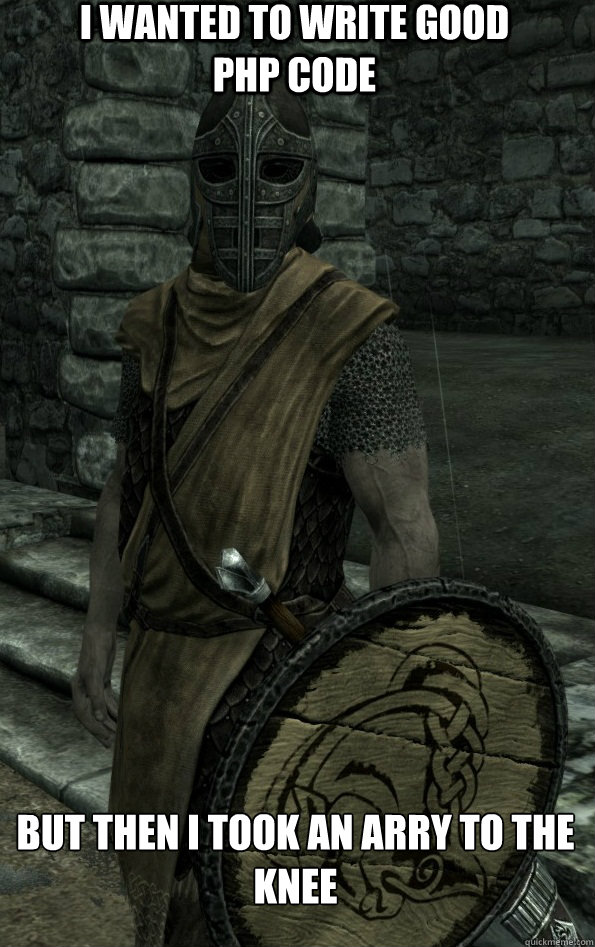
\includegraphics[height=200px]{./../graph/Meme/arraytotheknee.jpg}
\end{figure}
\end{center}
\end{frame}


\begin{frame}{comparing things}
\begin{center}
\begin{figure}[ht]
  \centering
	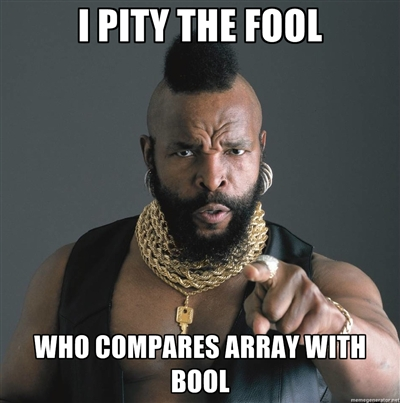
\includegraphics[height=200px]{./../graph/Meme/Mr_T.jpg}
\end{figure}
\end{center}
\end{frame}


\begin{frame}{comparing things}{one diamond hidden in php}
\begin{itemize}
	\item the comparision operator compares \textbf{and} converts things
	\begin{itemize}
		\item $123456$ == $" 123456"$
		\item $"1e3"$ == $"1000"$
		\item $"61529519452809720693702583126814"$   ==  $"61529519452809720000000000000000"$
		\item $array("foo","bar")$ == $true$
		\item $array()$ == $false$
	\end{itemize}
	\item All of above statements are evaluated as \textit{true} 
	\item '0' == false, 0.0 == false, '0,0' == true
\end{itemize}
\end{frame}


\begin{frame}{php is teached wrong}
\begin{itemize}
	\item An example of a php book
	\begin{enumerate}
		\item Learn ALL the features of php
		\item use them in examples
		\item and on the last page: the code in the examples isn't safe
	\end{enumerate}
	\item using obscure handlers instead of frameworks
	\item oop is teached the same way as your parents introduced you to your grandgrandgrand-mother
	\item php is often selfteached by bad examples found on strange webpages
\end{itemize}
\end{frame}

\begin{frame}{last slide of security problems}{as announced on the previous slide}
\begin{itemize}
\item the language it self (like any other) don't care about safe, secure and reliable code
\item it gives you freedom: if you want to write insecure code, just go an do it
\item $\Rightarrow$ a lot of php-applications on the web are \textbf{insecure} by default
	\begin{itemize}
		\item htmlentities
		\item input filters
		\item escaping the input
	\end{itemize}
\item \alert<2> { all userinput is evil }
\end{itemize}
\end{frame}

\begin{frame}
\begin{center}
\begin{figure}[ht]
  \centering
	
\includegraphics[height=150px]{./../graph/Meme/allthethings.jpg}
\end{figure}
\end{center}
\end{frame}



\begin{frame}{Conclusion}
\begin{itemize}
\item php isn't a bad language
\item yes, it has design flaws
\item using frameworks will reduce problems
\item \textbf{but} php makes it easy to do things wrong
\item so the user must take care about what he/she/it is doing.
\end{itemize}
\end{frame}

\begin{frame}
\begin{center}
\vspace{1em}
\hrule
\vspace{0.4em}
Questions?
\vspace{0.4em}
\hrule
\vspace{1em}
\end{center}
\end{frame}

\begin{frame}{last words}
\begin{center}
\vspace{1em}
\hrule
\vspace{0.4em}
don't \textit{think} or even \textit{assume} what php might do. \newline
just \alert<2>{\textbf{R}}ead \alert<2>{\textbf{T}}he \alert<2>{\textbf{F}}ucking \alert<2>{\textbf{M}}anual
\vspace{0.4em}
\hrule
\vspace{1em}
\end{center}
\end{frame}

\end{document}